\chapter{}

Voltei para a Bodoquena numa disposição incrível.
Agora mais do que nunca eu tinha que dar força ao meu companheiro.
Afinal, estava a caminho um herdeiro.
A felicidade estava completa e o futuro sorria.
Éramos donos de uma bela propriedade, num lugar belíssimo e Paulo se agigantava aos meus olhos no comando daquele monte de gente dando ordens, tomando decisões e aparentando uma calma e uma segurança de quem nunca tinha feito outra coisa na vida.
Dias depois, já instalada no meu modesto apartamento no barracão da Santa Teresa, pude acompanhar de perto os trabalhos da derrubada.

Os peões de derrubada se inscrevem numa categoria particular de trabalhadores.
São conhecidos também como ``peões de trecho'', uma massa sem rosto, sem passado e sem futuro, sem história, um dia aqui, outro ali, sempre na estrada, à cata de serviço.
No Mato Grosso daquela época, muitos eram índios, pela sua excepcional habilidade em lidar com o machado.
Outros eram foragidos da justiça, criminosos que se refugiavam no anonimato daquele serviço que os mantinha escondidos em acampamentos improvisados na floresta por meses a fio.
Todos estavam ali por falta de opção ou por terem se habituado àquela vida sem amarras.
Eram subordinados aos ``gatos'', homens duros e por vezes violentos que os recrutavam e garantiam que se mantivessem no trabalho até o fim da empreitada.


Da cabeça de um peão de trecho pode falar um episódio que se deu entre Paulo e um deles, o Guanayr.
Este tinha pegado por empreita um pedaço do fundo da fazenda e tinha uma característica especial: não estava ligado a nenhum gato.
Foi dos poucos que trouxe a família com ele.
Mulher, e filho, e mais um ou dois ajudantes, arranchados sob um barraco de palha no meio da mata.
Alto, moreno, magro, de pouco falar e um jeito meio abusado.
Um dia, Paulo deu pela sua ausência.
Tinha saído sem avisar, acho.
Quando voltou, foi chamado às falas.
Ouviu calado.
Quando Paulo acabou, Guanayr tomou a palavra, naquele seu jeito pausado:
\textit{``-- Doutor, o senhor me desculpe, mas não gosto que falem comigo desse jeito.
Faço meu trabalho direito, cumpro o que trato, mas não tenho dono, não.
O senhor pode ser rico, tem essa fazenda, e por isso mesmo está preso aqui, não é? Pois eu sou mais rico, porque sou livre.
O que eu tenho cabe no chapéu e nada me segura em lugar algum.
Sou livre para ir para onde quiser, qualquer lugar desse mundo é meu, porque em qualquer lugar eu acho pouso e trabalho.
Se não gostou de alguma coisa é só dizer que eu vou-me embora agora mesmo.
Sem nenhum problema.''}
 
Nem preciso dizer que não foi porque conquistou nossa completa admiração, formou o mais bonito talhão de café da Santa Teresa e foi embora quando quis.
Altivo e calado, como sempre.

\begin{figure}
\centering
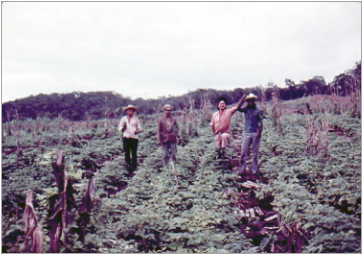
\includegraphics[width=0.8\linewidth]{22/guanayr.png}
\caption{Guanayr, último à direita, no seu talhão de café.}
\end{figure}

Mas, nem todos eram como Guanayr.
Um dia, estávamos ali perto do barracão eu e meu guarda-costas, o velho Tibúrcio, porque desde que a turma da derrubada se instalara fazenda ele não saía do meu lado de manhã até à noite, quando a voz alterada do Paulo se fez ouvir um pouco além da porteira que abria para os fundos da fazenda.
Olhando naquela direção, nós o vimos trazendo um dos peões aos sopapos pela estrada.
Parecia tão bravo que nem ouvia os nossos chamados.
Passou adiante, sem parar com os pescoções até jogar o infeliz para fora da fazenda e bater com a porteira lá da entrada.
Atônitos, ficamos aguardando sua volta.
Chegou já reinstalado na sua calma habitual e se limitou a dizer que o sujeito tinha querido enfrentá-lo.
Tibúrcio se inflamou.
Paulo havia tomado a arma dele por precaução, porque quando o velho bugre bebia, lembrava-se dos seus tempos de justiceiro e começava a chamar todo mundo para briga, querendo atirar para todo lado, um reboliço danado.
Mas agora, com um cabra perigoso como aquele que o Paulo acabara de tocar dali, não tinha jeito, ele tinha que ter a arma de volta, implorava Tibúrcio.
Paulo recusou e saiu sorrindo, de volta para o trabalho.
O velho ficou inconformado.
A moça que me ajudava na casa puxou-me para o lado, com expressão alarmada: 
\textit{``-- Escute, Dona Teresa, o Doutor vai mesmo precisar tomar cuidado.
Aquele homem que ele botou para fora está fugido da polícia.
É matador conhecido por aqui.
É bem capaz de voltar para se vingar''}.


Poucos dias depois, já escurecendo, voltávamos Paulo, eu e Tibúrcio de Bonito quando, um pouco antes da entrada da fazenda, demos com um pesado tronco atravessado como que de propósito no meio da estrada.
Ressabiados, os dois desceram da caminhonete para remover o obstáculo.
Quando retornou ao volante, Paulo não pode conter o riso.
Deu comigo, grávida, olhos arregalados, segurando com as duas mãos o seu Colt 38 e apontando-o em todas as direções, pronta para repelir a emboscada.
Isso, claro, se eu soubesse atirar.
Como não sabia, Paulo aconselhou-me a guardá-lo antes que acabasse matando um de nós.

Uma manhã, Tibúrcio e eu fomos andar pela derrubada, a cavalo.
Eu na frente, ele atrás, proseando.

\textit{``-- Tibúrcio, é verdade que você matou um monte de gente fazendo justiça aqui pela Bodoquena?'' }

\textit{``-- Dona Teresa, aqui justiça era muito difícil.
De longe em longe, aparecia na vila um juiz que vinha de Aquidauana.
Mas, pelo resto do tempo, não havia quem defendesse essa terra de malfeitor e isso a senhora sabe que aparece em todo lugar.
Essa gente toda ficava muito desprotegida.
Então, alguém tinha que fazer o serviço.
Agora, eu lhe digo uma coisa, nunca matei ninguém que eu não tivesse certeza que merecia morrer.
Aqui mesmo onde estamos, nessa parte de cima da fazenda, deu-se um fato que eu vou contar para a senhora saber que estou dizendo a verdade: 
um fazendeiro me contratou para matar um advogado.
Disse que esse moço que era de fora, um paulista, tinha sido desonesto num negócio que tinham feito, e ainda por cima andara se engraçando com a mulher dele.
Não tinha perdão.}

\textit{Arrumei um jeito de trazer o rapaz até aqui, com a história de lhe mostrar a fazenda, pois ele estava pensando em comprar uma.
A cavalo, como eu e a senhora estamos agora, ele na frente e eu atrás, comecei a puxar conversa, querendo saber quem ele era, de onde vinha, fazer o quê e aí por diante.
Era um costume que eu tinha, antes de cumprir o trato, para ter certeza que o infeliz merecia o destino.
O moço, então, começou a falar da vida que levava, da profissão, da mulher, dos filhos e quando contou o que tinha vindo fazer por estas bandas e o negócio que o tal fazendeiro tinha lhe proposto, tive a certeza de que aquele maldito, o que me contratou, tinha mentido.
Levei o moço de volta para o povoado, virei o cavalo nos cascos, fui lá e matei o fazendeiro.''}

Todo dia, cedo, Tibúrcio me trazia coalhada.
Fresquinha.

\textit{``-- Para o menino nascer forte. É bom.''}

\textit{``-- Tibúrcio, me ajude a fazer uma horta.''}
Lá fomos nós, mais ele do que eu, levantar a cerca, construir os canteiros, fazer as mudas com as sementes que eu trouxera de Campo Grande.

Semanas depois, amarrávamos os pés de tomate nas estacas para levantá-los do chão, quando Tibúrcio começou a insistir:

\textit{``-- Dona Teresa, deixe isso e vá já para dentro.
O sol está muito quente para o menino''}

\textit{``-- Que nada, Tibúrcio, com esse friozinho, está até bom.''}

\textit{``-- Saia daí, Dona Teresa, a senhora não está fazendo direito, vai matar as plantas apertando assim.''}

Teimei:
\textit{``-- Não estou apertando nada, venha ver.''}

\textit{``-- Olhe, lá vem Doutor Paulo, vai ficar bravo em lhe ver agachada nessa posição!''}

Virei o rosto na direção indicada.
Certeiro, o velho ergueu o facão e decapitou a jararaca enrodilhada sob o pé de tomate, a dois passos de onde eu estava.

Quando a derrubada terminou, já fazia muito frio na serra.
A madeira estava toda enleirada, pronta para queimar.
À noite, naquele barracão de madeira, o vento passava pelas frestas e cortava como lâmina de gelo.
Dormíamos, Paulo e eu, vestidos e calçados de bota e tudo sob os cobertores, agarrados um ao outro e nos virávamos em ordem unida, para não esfriar a parte do corpo já aquecida.


Certa madrugada fomos subitamente despertos por um tropear e um relinchar medonhos, seguidos de tão fortes pancadas na parede do barracão que pareciam querer pô-lo abaixo.
De novo agarrei o 38 que estava à mesa de cabeceira e me preparei para o ataque.
Paulo, estremunhado, escutou por um momento e, tirando o revólver da minha mão, disse:
\textit{``-- É o bagual, sossegue.''}

Esse potro, um belo animal até, Benício deixou para trás porque surgira na fazenda não se sabe como e ninguém deu conta de domá-lo.
Surgia e desaparecia conforme lhe dava na veneta.
Mas, a partir de quando Paulo ordenou que recolhessem os animais mansos no piquete, à noite, o bicho pareceu se sentir desafiado.
Deu para se exibir por ali em atitudes atrevidas, empinando nas patas traseiras, balançando as longas crinas e relinchando provocadoramente como se zombasse daqueles infelizes submissos, presos dentro do cercado.
Parecia querer incitá-los à fuga e à liberdade.
Os pobres coitados se agitavam, para lá e para cá, sem coragem ou sem saber como e o espetáculo se repetia, noite, após noite.
Até que, naquela ocasião, o bagual passou da provocação à ação, decidindo, ao que parece, arrebentar o piquete.
Foi o fim da sua carreira de agitador.
No dia seguinte, Paulo determinou a caça ao rebelde.
Laçado e trazido à força para o pasto, foi confiado a Felipe, um domador profissional.
Não sei se algum dia o bagual aceitou a sela.
Paulo diz que sim.
Mas deve ter demorado, porque até quando não pude mais viajar para a fazenda, no fim da gravidez, nunca vi ninguém montá-lo por mais que alguns minutos.

\begin{figure}
\centering
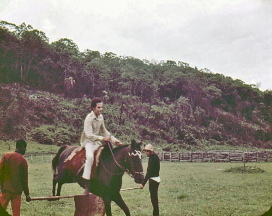
\includegraphics[width=0.8\linewidth]{22/paulo+bagual.png}
\caption{Paulo montando o bagual.}
\end{figure}

\begin{figure}
\centering
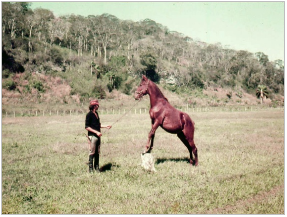
\includegraphics[width=0.8\linewidth]{22/bagual+felipe.png}
\caption{O bagual e Felipe, o domador.}
\end{figure}